\documentclass[geometry-lectures-19.tex]{subfiles}
\begin{document}

\section{Symplectic geometry}

A symplectic form on a smooth manifold $M$ is non-degenerate closed 2-form $\omega$. ``Non-degenerate'' means that the mapping $\omega : TM \to T^*M$; $X \mapsto \omega(X,-)$
 is an isomorphism. We denote the 1-form $\omega(X,-)$ by $i(X)\omega$.


 The couple ($M, \omega$) of a smooth manifold $M$ and a symplectic form $\omega$ is called a
\textbf{symplectic manifold}. Any symplectic manifold is even dimensional and if dim($M) =
2n$, $\omega^n$ is a volume-form.


 \bexample
 Let $(q_1,\cdots, q_n,p_1,\cdots, p_n)$ be the standard coordinate of $\R^{2n}$. Then,
 $$
\omega=\sum_{i=1}^n dq_i\wedge dp_i~
 $$
 is the symplectic form.
 \eexample

  \bexample[cotangent bundle]
A symplectic manifold $(M,\omega)$ is called \textbf{exact} if there exists one form $\theta$ such that $\omega=d\theta$ where $\theta$ is called \textbf{Liouville 1-form}. The  vector field $Z$ dual to the Liouville 1-form with respect to $\omega$
$$
i_Z\omega=\theta
$$
is called  \textbf{Liouville vector field}. The most important example of exact symplectic manifolds is a cotengent bundle $M=T^*N$ of a smooth manifold $N$. Given a local coordinate $(q_1,\cdots,q_n)$, they induces the coordinate $(p_1,\cdots,p_n)$ on the fiber $T^*_qN$. Then, the Liouville 1-form is written in terms of the local coordinate of $T^*N$
$$
\theta=\sum_{i=1}^np_id q_i
$$
so that the symplectic form can be locally written as
$$
\omega=\sum_{i=1}^n dq_i\wedge dp_i~.
$$
 \eexample

 \bexample
 A K\"ahler manifold is a symplectic manifold $(M,\omega)$ equipped with an integrable almost-complex structure $J$ which is compatible with the symplectic form $\omega$, meaning that the bilinear form
$$g(u,v)=\omega (u,Jv)$$
on the tangent space of $M$ at each point is symmetric and positive definite (and hence a Riemannian metric on $M$).
 \eexample



  \bthm[Darboux's theorem]
Let $(M, \omega)$ be a $2n$-dimensional symplectic manifold,
and let $p$ be any point in $M$.
Then there is a coordinate chart $(U, q_1,\cdots , q_n,p_1,\cdots,p_n)$ centered at $p$ such that
on $U$
\be\label{symp}\omega=\sum_{i=1}^n dq_i\wedge dp_i~.\ee
 \ethm

This theorem states that any symplectic manifold is locally equivalent
to an Euclidean space with its standard symplectic structure. As a result, the most
important questions in symplectic geometry are the global ones.


\subsection{Symplectomorphisms}

 The important maps in symplectic topology are the \textbf{symplectomorphisms}. A symplectomorphism
between two symplectic manifolds $(M, \omega_M)$ and $(N, \omega_N )$ is a diffeomorphism
$\psi : M\to N$ such that
$$
\psi^\ast \omega_N=\omega_M~.
$$
In fact, this condition is pretty strong. The necessary condition for the existence of symplectomorphisms is $\dim M \le\dim N$.

  \bexample[symplectic group]
Let $E = \R^{2n}$ with basis $\{e_1,\cdots ,e_n,f_1,\cdots ,f_n\}$. Then
$$\omega(e_i,e_j ) = 0~,\quad \omega(f_i,f_j ) = 0~,\quad \omega(e_i
,f_j ) = \delta_{i,j}~ .$$
defines a symplectic structure on $E$. Then,  examples of symplectomorphisms are
$$
Sp(E,\omega)=\{g\in GL(2n,\R) ~|g^TJg=J ~, \quad J=\begin{pmatrix}0&I_n\\-I_N&0\end{pmatrix}\}
$$
which is called the \textbf{symplectic group}.
 \eexample



  \bthm[Moser Stability Theorem] Let $(M, \omega_t)$ be a closed manifold with a family of
cohomologous symplectic forms. Then there is a family of symplectomorphisms $\psi_t
: M \to M$
such that
$$\psi_0 = 1~, \psi^*_t \omega_t = \omega_0~.$$
Moreover, if $\omega_t (q) = \omega_0 (q)$ for all points $q$ on a compact submanifold $Q$ of $M$, we may
assume $\psi_t$ is the identity on $Q$.
 \ethm


This theorem says that one cannot change the symplectic form in any important
way by deforming it, provided that the cohomology class is unchanged.

 \subsection{Lagrangian submanifolds}

  \bdefn[Lagrangian submanifold]
A Lagrangian submanifold of a sympletic manifold $(M,\omega )$ is a submanifold where the restriction of the symplectic form $\omega$  to $L\subset M$ is vanishing, i.e. $\omega |_{L}=0$ and ${\text{dim }}L=1/2\cdot {\text{dim }}M$.
\edefn

If we perturb a Lagrangian submanifold, then it is no longer Lagrangian in general. Thus, they are ``rigid'' objects in symplectic geometry. Since Lagrangian submanifolds play very important role in symplectic geometry, Weinstein advertised slogan that everything is a Lagrangian submanifold. (A. Weinstein's lagrangian creed.)

  \bexample
The zero section $N$ of the cotangent bundle $M=T^*N$ is a Lagrangian submanifold. Let $f:Z\hookrightarrow N$ is an embedding. Then, the conormal bundle to $Z$ in $T^*N$ defined as
$$L_Z:=\{(x,\alpha)\in T^*N| x\in Z~, \quad \alpha(v)=0~ \textrm{for all}~ v\in T_xZ\}\subset T^*N~,$$
is a Lagrangian submanifold.
\eexample

It is known that the neighborhood of a Lagrangian also has the standard symplectic structure as its cotangent bundle.

  \bthm[Weinstein's tubular neighbourhood theorem]
Every lagrangian submanifold $L$ in a symplectic manifold $(M,\omega)$ has a neighbourhood $U$ which is symplectomorphic to a neighbourhood $V$ of the zero section of the cotangent bundle $T^*L$.
\ethm

  \subsection{Hamiltonian system}

 Any smooth function $H\in C^\infty(M)$ gives rise to a vector field $X_H$ defined uniquely
by the equation
$$i(X_H)\omega = dH~.$$
This vector field is called the \textbf{Hamiltonian vector field} with Hamiltonian $H$. Given a symplectic form \eqref{symp},
the flow of the Hamiltonian vector field $X_H$ associated to a Hamiltonian $H$ can be described by
$$
\frac{dq_i}{dt}=\frac{\partial H}{\partial  p_i}~,\qquad \frac{dp_i}{dt}=-\frac{\partial H}{\partial  q_i}~,
$$
which are Hamilton's canonical equations.

For $f,g\in C^\infty(M)$, we define the Poisson product by
$$
\{ f,g\}=\omega(X_f,X_g)=X_f(g)=-X_g(f)~.
$$
Given the symplectic form \eqref{symp}, the Poisson product can be written as the local coordinate
 $$
 \{ f,g\}=\sum_{i=1}^n \left(\frac{\partial f}{\partial  q_i}\frac{\partial g}{\partial  p_i}-\frac{\partial f}{\partial  p_i}\frac{\partial g}{\partial  q_i} \right)~.
 $$
 They satisfy the following properties
 \begin{description}
\item{Skew symmetry:} $ \{f,g\}=-\{g,f\}.$
\item{Jacobi identity:} $ \{f,\{g,h\}\}+\{g,\{h,f\}\}+\{h,\{f,g\}\}=0.$
\item{Leibniz's Rule:} $ \{fg,h\}=f\{g,h\}+g\{f,h\}.$
\end{description}
Using these properties, one can show that
$$
[X_f,X_g]=X_{\{f,g\}}~.
$$
 For $f\in C^\infty(M)$,  the differentiation with respect to the Hamiltonian flow  can be expressed by
 $$
 \frac{df}{dt}=-\{H,f\}~.
 $$
If $\{f,H\}=0$, the flow generated by $X_f$ is a symmetry of the Hamiltonian system with $H$. Namely, if we denote the flow by $\varphi_s$, then we have
$$
\frac{dH}{ds}=\{f,H\}=0~,
$$
 or equivalently,
 $$
 \frac{df}{dt}=-\{H,f\}=0~.
 $$
This is called \textbf{Noether theorem.}


\bexample
If they system has spherical symmetry, the potential $V(r)$ is independent of $\theta$ and $\phi$. Then, the momenta $p_\theta$ and $p_\phi$ are conserved.
\eexample




 \subsection{Arnold-Liouville theorem}
Let us consider Poisson commuting functions (Hamiltonians)
$H_1, \cdots , H_k$  with $\{H_i, H_j\} = 0$ for all $i, j$. To insure that we are not discussing a degenerate situation, we assume that
$dH_1\wedge \cdots \wedge dH_k(x) \neq 0$ for $\forall x\in M$, in which $H_i$ are called  \textbf{analytically independent}. Then, the maximal number of Poisson commuting functions is a half of dimension of $M$ which is $n$. An $2n$-dimensional symplectic manifold $(M,\omega)$ with $n$ Poisson commuting Hamiltonians is called \textbf{completely integrable system}.


\bthm[Arnold-Liouville theorem]
Let $H_1, \cdots , H_n$ be a completely integrable system on a $2n$-dimensional symplectic manifold  $(M,\omega)$. Namely,
$\pi=(H_1, \cdots , H_n):M\to \R^n$ are analytically independent Poisson commuting functions with $\{H_i, H_j\} = 0$ for all $i, j$. Then, a compact connected component of the preimage of a non-singular point of $\pi$ is a Lagrangian submanifold that is diffeomorphic to a torus $T^n$.
\ethm

Let us denote the image of $\pi$ by $B$. Then, (compact connected component  of) the preimage $L=\pi^{-1}(b)$ of $b\in B$ is diffeomorphic to $T^n$ so that we can take the angle coordinate
$$
(\phi_1\cdots \phi_n):	L\to T^n
$$
We can further take local coordinate $(I_1,\cdots,I_n)$ of $B$ that the symplectic form can be locally expressed as
$$
\omega=\sum_{i=1}^n d\phi_i\wedge dI_i~,
$$
where $(\phi_i,I_i)$ are called \textbf{angle-action} coordinate.



\bexample
  Consider the harmonic oscillator with Hamiltonian
  \[
    H(q, p) = \frac{1}{2}p^2 + \frac{1}{2}\omega^2 q^2.
  \]
  Since is a 2-dimensional system, so we only need a single first integral. Since $H$ is a first integral for trivial reasons, this is an integrable Hamiltonian system.

  We can actually draw the lines on which $H$ is constant --- they are just ellipses:
  \begin{center}
    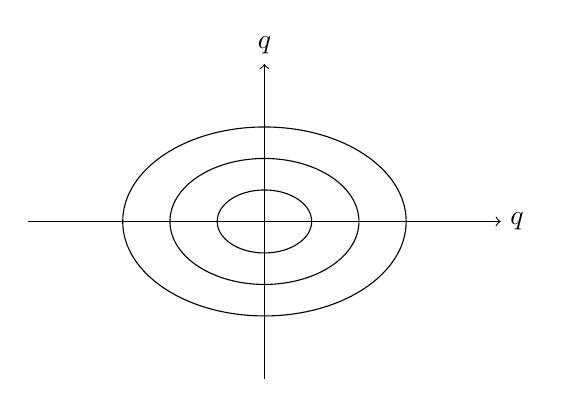
\begin{tikzpicture}
      \draw [->] (-3, 0) -- (3, 0) node [right] {$q$};
      \draw [->] (0, -2) -- (0, 2) node [above] {$q$};

      \foreach \x in {0.4, 0.8, 1.2} {
        \begin{scope}[scale=\x]
          \draw ellipse (1.5 and 1);
        \end{scope}
      }
    \end{tikzpicture}
  \end{center}
  We note that the ellipses are each homeomorphic to $S^1$. Now we introduce the coordinate transformation $(q, p) \mapsto (\phi, I)$, defined by
  \[
    q = \sqrt{\frac{2I}{\omega}} \sin \phi,\quad p = \sqrt{2I\omega} \cos \phi,
  \]
Hence, $\phi$ is the angle coordinate that parametrizes $S^1$ in the Arnold-Liouville theorem.

  We can manually show that this transformation is canonical, but it is merely a computation and we will not waste time doing that. In these new coordinates, the Hamiltonian looks like
  \[
    \tilde{H}(\phi, I) = H(q(\phi, I), p(\phi, I)) = \omega I.
  \]
The Hamiltonian is independent of $\phi$! Therefore, the Hamilton equations become
  \[
    \dot\phi = \frac{\partial \tilde{H}}{ \partial I} = \omega,\quad \dot{I} = -\frac{\partial \tilde{H}}{\partial \phi} = 0.
  \]
  We can integrate up to obtain
  \[
    \phi(t) = \phi_0 + \omega t,\quad I(t) = I_0.
  \]
It is interesting to consider the integral along paths of constant $H$:
  \begin{align*}
    \frac{1}{2\pi}\oint p \;\d q &= \frac{1}{2\pi} \int_0^{2\pi}p(\phi, I) \left(\frac{\partial q}{\partial \phi} \;\d \phi + \frac{\partial q}{\partial I} \;\d I\right)\\
    &= \frac{1}{2\pi} \int_0^{2\pi}p(\phi, I) \left(\frac{\partial q}{\partial \phi} \;\d \phi\right)\\
    &= \frac{1}{2\pi} \int_0^{2\pi} \sqrt{\frac{2I}{\omega}}\sqrt{2I\omega} \cos^2 \phi \;\d \phi\\
    &= I~.
  \end{align*}
We could always have performed the integral $\frac{1}{2\pi} \oint p \;\d q$ along paths of constant $H$ without knowing anything about $I$ and $\phi$, and this would have magically gave us the new coordinate $I$. That's why it is called \textbf{integrable system}.
\eexample












%
%
%\begin{thebibliography}{99}

%\bibitem{Candelas}
%P. Candelas, X. C. de La Ossa, P. S. Green, L. Parkes, \textit{A pair of Calabi-Yau manifolds as an exactly soluble superconformal theory}. Nucl.Phys. B359 (1991) 21-74.
%
%\bibitem{Bouchard}
%Vincent. Bouchard,  \textit{Lectures on complex geometry, Calabi-Yau manifolds and toric geometry.} \href{http://arxiv.org/abs/hep-th/0702063}{hep-th/0702063} (2007).
%
%\bibitem{Calabi-Yau}
%Calabi-Yau manifolds,
%\url{http://www.scholarpedia.org/article/Calabi-Yau_manifold}
%
%\end{thebibliography}


\end{document}
